\documentclass{article}
% Allows control of page geometry
% Set to 1 inch margins (mla standard I guess)
\usepackage[margin=1in]{geometry}

% Graphics package
% Use it like:
% \begin{figure}[H]
% \centering
% \includegraphics[width=90mm,angle=0]{fixed_dome1.jpg}
% \caption{A simple caption}
% \label{overflow}
% \end{figure}	
\usepackage[pdftex]{graphicx}

% Allows you to include pdf documents or pages in the document
% using \includepdf[pages=2-4]{file} or whatever 
\usepackage{pdfpages}

% Self explanatory, appendix package
\usepackage{appendix}

% The listings package is used for inserting source code with highlights
\usepackage{listings}
\usepackage{color}
\lstdefinestyle{custom}{
  belowcaptionskip=1\baselineskip,
  language=bash,
  showstringspaces=false,
  basicstyle=\footnotesize\ttfamily,
  keywordstyle=\bfseries\color{green!40!black},
  commentstyle=\itshape\color{purple!40!black},
  identifierstyle=\color{blue},
  stringstyle=\color{orange},
  numberstyle=\ttfamily
}
\lstset{style=custom}

% Hyperref package is used for hyperlinking the document (ex: toc links)
\usepackage{hyperref}
\hypersetup{
    colorlinks,
    citecolor=black,
    filecolor=black,
    linkcolor=black,
    urlcolor=black
}

\usepackage{float}
\restylefloat{figure}

% Title Page
\title{CAN-obd2}
\author{Kevin Krieger}
\date{January 2014}

\begin{document}
\maketitle
\tableofcontents
\newpage

\section{History} \label{history}

\subsection{Version 1}

\begin{figure}[H]
\centering
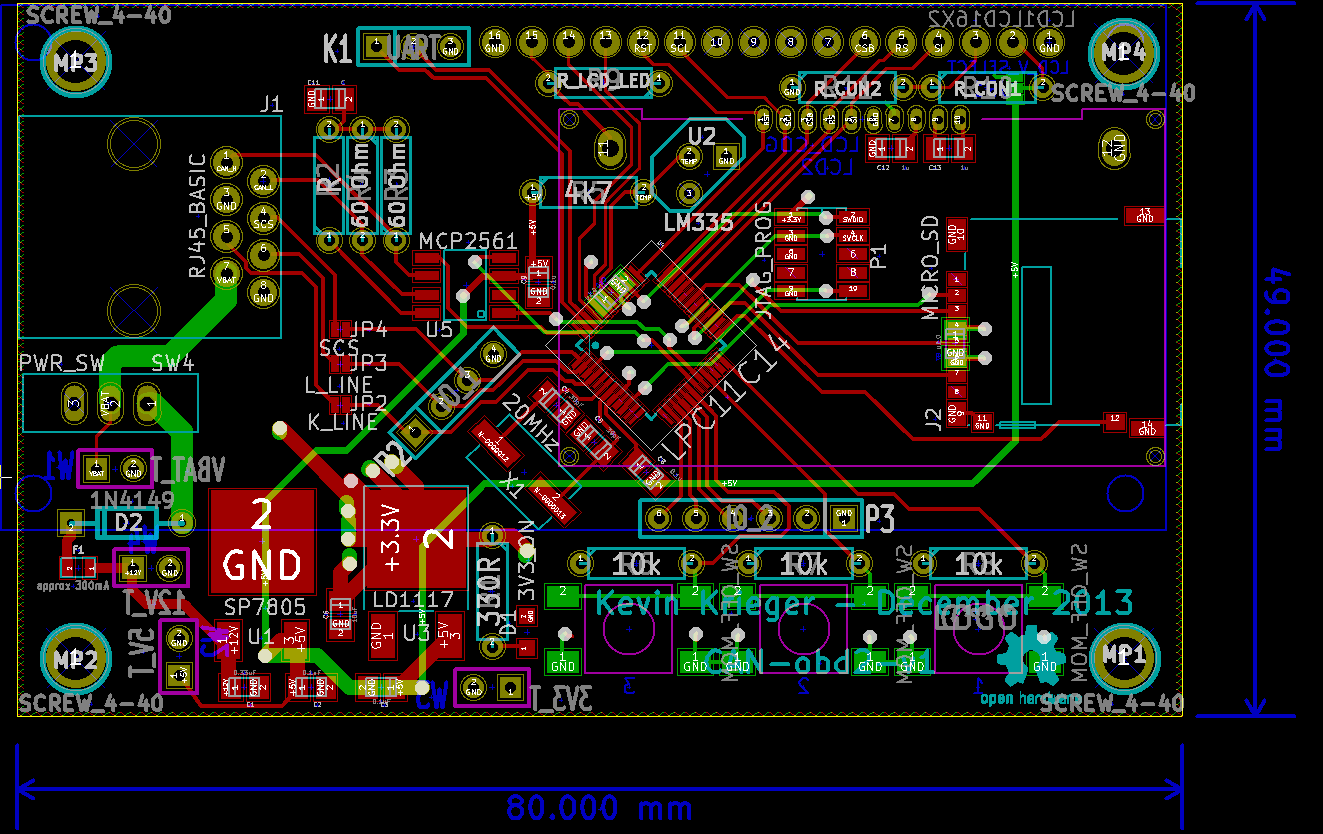
\includegraphics[width=180mm,angle=90]{../images/board_layout.png}
\caption{Board layout - Kicad}
\label{}
\end{figure}

\begin{figure}[H]
\centering
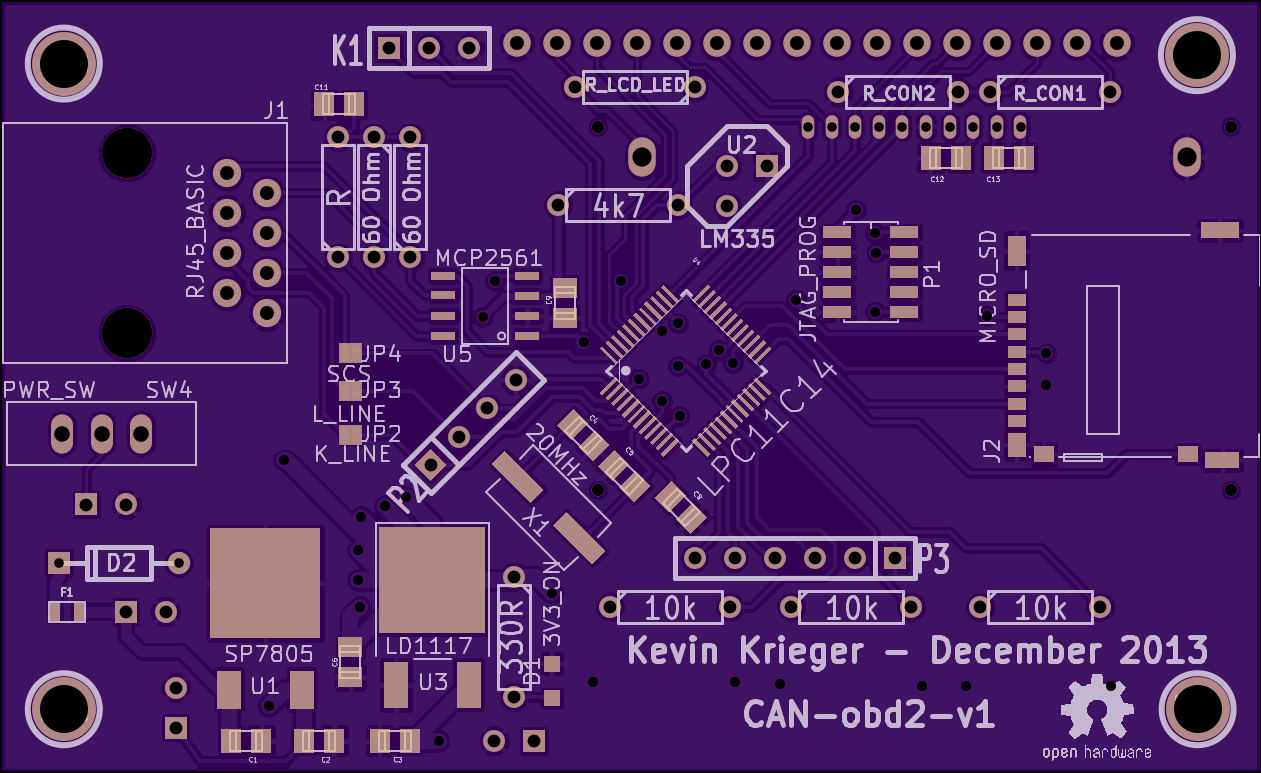
\includegraphics[width=180mm,angle=90]{../images/canobd2v1top.png}
\caption{oshpark.com top render}
\label{}
\end{figure}

\begin{figure}[H]
\centering
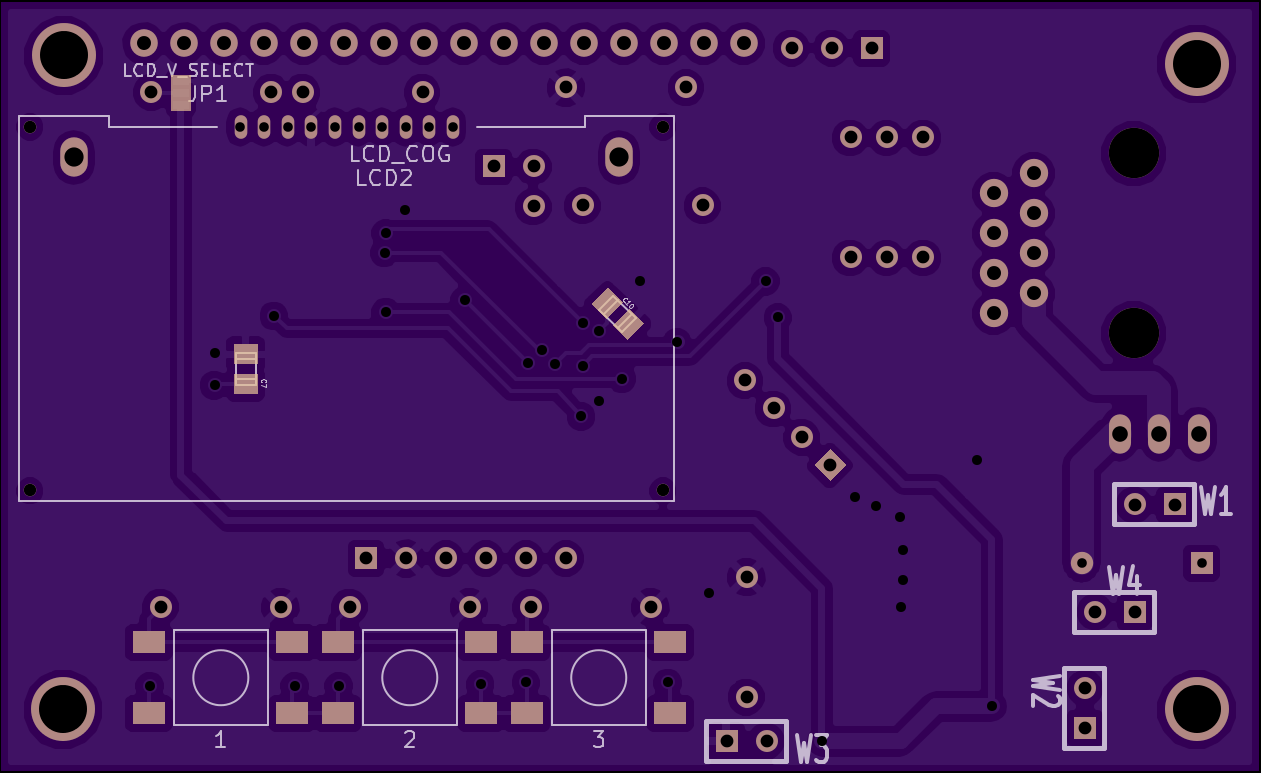
\includegraphics[width=180mm,angle=90]{../images/canobd2v1bot.png}
\caption{oshpark.com bottom render}
\label{}
\end{figure}

\begin{figure}[H]
\centering
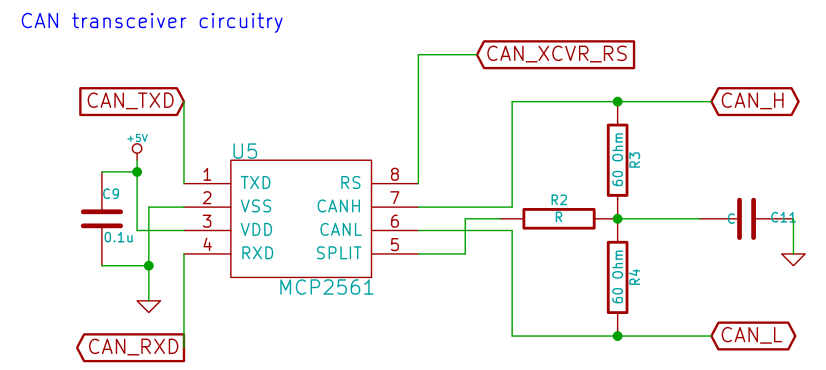
\includegraphics[width=140mm,angle=0]{../images/can_transceiver.png}
\caption{CAN transceiver circuitry}
\label{}
\end{figure}

\begin{figure}[H]
\centering
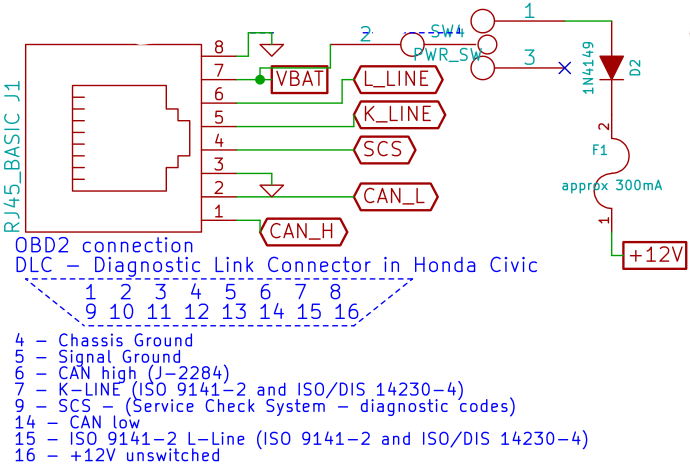
\includegraphics[width=140mm,angle=0]{../images/car_interface.png}
\caption{Interface to automobile data port (2008 Honda Civic)}
\label{}
\end{figure}

\begin{figure}[H]
\centering
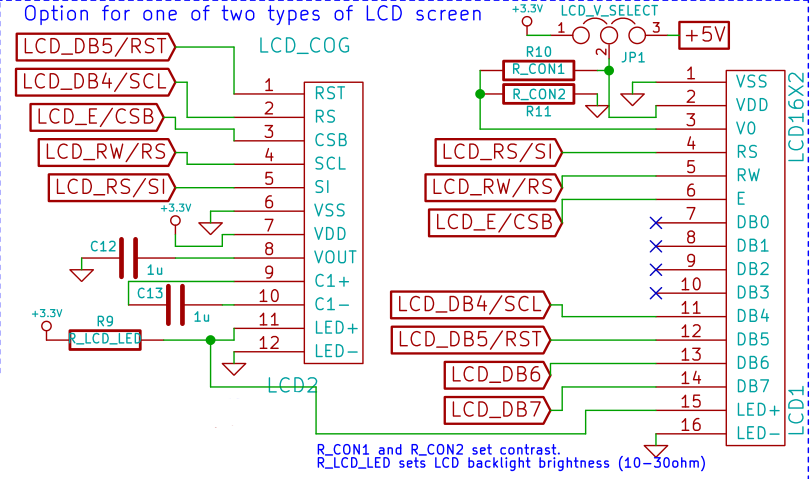
\includegraphics[width=140mm,angle=0]{../images/lcd_screens.png}
\caption{Two LCD screen options - circuitry}
\label{}
\end{figure}

\begin{figure}[H]
\centering
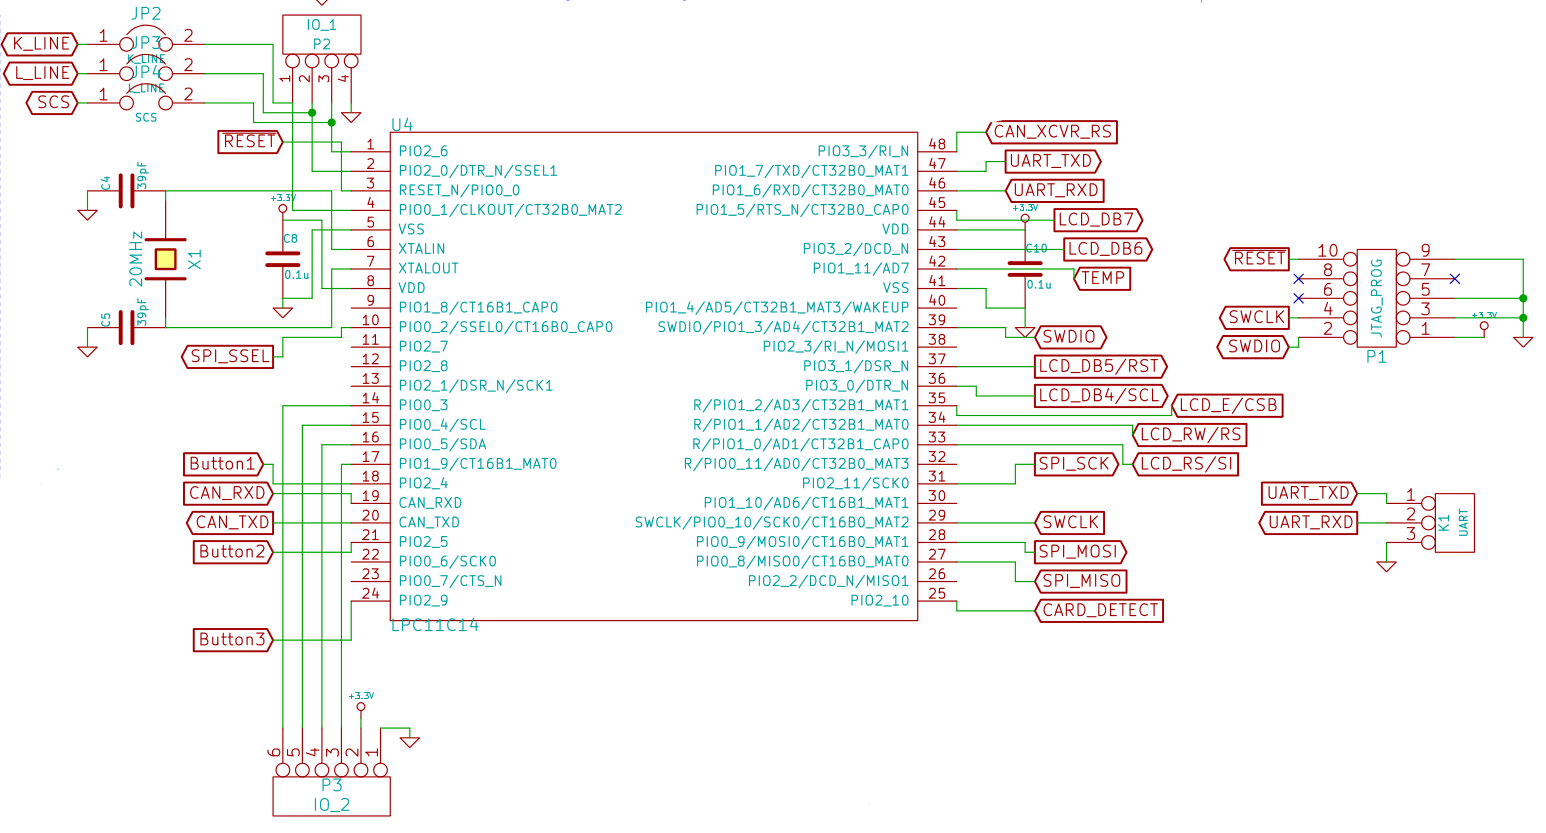
\includegraphics[width=140mm,angle=0]{../images/micro.png}
\caption{Microcontroller circuitry, IO connectors and programming port}
\label{}
\end{figure}

\begin{figure}[H]
\centering
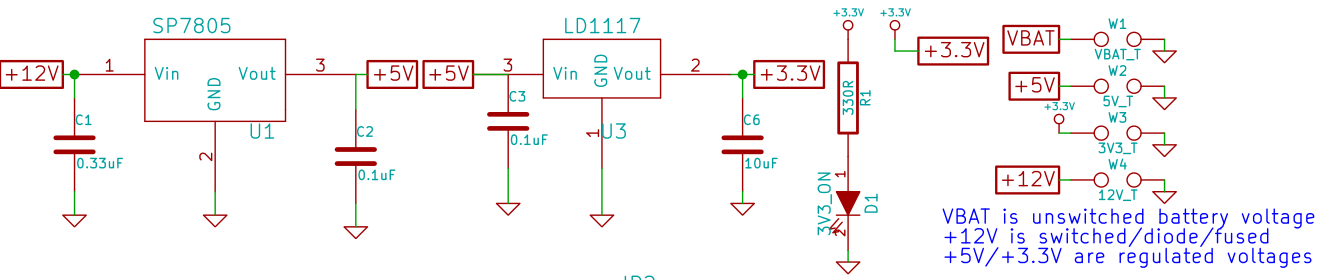
\includegraphics[width=140mm,angle=0]{../images/pwr_and_test.png}
\caption{Power and test point circuitry}
\label{}
\end{figure}

\begin{figure}[H]
\centering
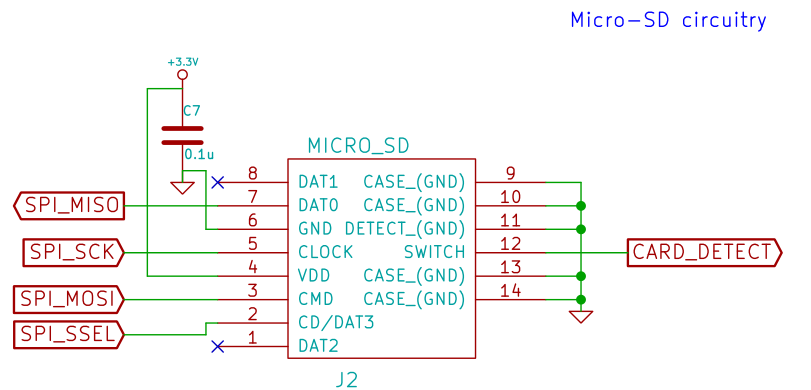
\includegraphics[width=140mm,angle=0]{../images/sd_card.png}
\caption{Micro SD card circuitry - SPI mode}
\label{}
\end{figure}

\begin{figure}[H]
\centering
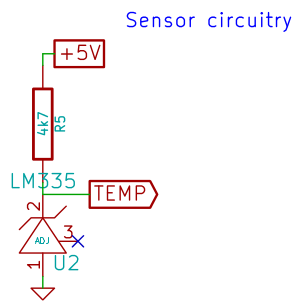
\includegraphics[width=140mm,angle=0]{../images/temp.png}
\caption{Temperature sensor circuit}
\label{}
\end{figure}

\begin{figure}[H]
\centering
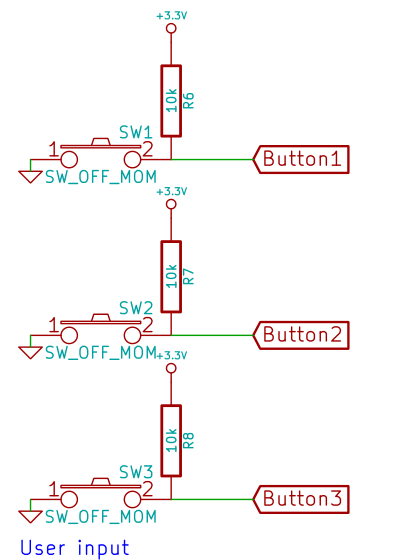
\includegraphics[width=140mm,angle=0]{../images/userinput.png}
\caption{User input circuitry}
\label{}
\end{figure}


\section{} \label{}

\section{} \label{}

\section{} \label{}

\section{} \label{}

\section{} \label{}

\section{} \label{}

%{%
%\newcommand{\mc}[3]{\multicolumn{#1}{#2}{#3}}
%\begin{center}
%\begin{tabular}[c]{|l|l|l|l|}\hline
%\mc{1}{|c|}{\textbf{Column 1}} & \mc{1}{c|}{\textbf{2}} & \mc{1}{c|}{\textbf%{3}} & \mc{1}{c|}{\textbf{4}}\\\hline
%Blah & Blah & blah 3 & \\
%Saskatchewan & Kevin Krieger & kevin.krieger@usask.ca & no info\\
%& & not much here &\\
%\hline
%\end{tabular}
%\end{center}
%}%

%{\bf THIS TEXT WILL BE LOUD!}

%\subsubsection{Subsubsection} \label{Labelsubsubsection}
%See the  \hyperref[overview]{Overview} section.

\appendix

\end{document}          
